\documentclass{beamer}

\pdfmapfile{+sansmathaccent.map}


\mode<presentation>
{
	\usetheme{Warsaw} % or try Darmstadt, Madrid, Warsaw, Rochester, CambridgeUS, ...
	\usecolortheme{seahorse} % or try seahorse, beaver, crane, wolverine, ...
	\usefonttheme{serif}  % or try serif, structurebold, ...
	\setbeamertemplate{navigation symbols}{}
	\setbeamertemplate{caption}[numbered]
} 


%%%%%%%%%%%%%%%%%%%%%%%%%%%%
% itemize settings


%%%%%%%%%%%%%%%%%%%%%%%%%%%%
% itemize settings

\definecolor{myhotpink}{RGB}{255, 80, 200}
\definecolor{mywarmpink}{RGB}{255, 60, 160}
\definecolor{mylightpink}{RGB}{255, 80, 200}
\definecolor{mypink}{RGB}{255, 30, 80}
\definecolor{mydarkpink}{RGB}{155, 25, 60}

\definecolor{mypaleblue}{RGB}{240, 240, 255}
\definecolor{mylightblue}{RGB}{120, 150, 255}
\definecolor{myblue}{RGB}{90, 90, 255}
\definecolor{mygblue}{RGB}{70, 110, 240}
\definecolor{mydarkblue}{RGB}{0, 0, 180}
\definecolor{myblackblue}{RGB}{40, 40, 120}

\definecolor{myblackturquoise}{RGB}{5, 53, 60}
\definecolor{mydarkdarkturquoise}{RGB}{8, 93, 110}
\definecolor{mydarkturquoise}{RGB}{28, 143, 150}
\definecolor{mypaleturquoise}{RGB}{230, 255, 255}
\definecolor{myturquoise}{RGB}{48, 213, 200}

\definecolor{mygreen}{RGB}{0, 200, 0}
\definecolor{mydarkgreen}{RGB}{0, 120, 0}
\definecolor{mygreen2}{RGB}{245, 255, 230}

\definecolor{mygrey}{RGB}{120, 120, 120}
\definecolor{mypalegrey}{RGB}{160, 160, 160}
\definecolor{mydarkgrey}{RGB}{80, 80, 160}

\definecolor{mydarkred}{RGB}{160, 30, 30}
\definecolor{mylightred}{RGB}{255, 150, 150}
\definecolor{myred}{RGB}{200, 110, 110}
\definecolor{myblackred}{RGB}{120, 40, 40}

\definecolor{mygreen}{RGB}{0, 200, 0}
\definecolor{mygreen2}{RGB}{205, 255, 200}

\definecolor{mydarkcolor}{RGB}{60, 25, 155}
\definecolor{mylightcolor}{RGB}{130, 180, 250}

\setbeamertemplate{itemize items}[default]

\setbeamertemplate{itemize item}{\color{myblackturquoise}$\blacksquare$}
\setbeamertemplate{itemize subitem}{\color{mydarkdarkturquoise}$\blacktriangleright$}
\setbeamertemplate{itemize subsubitem}{\color{mygray}$\blacksquare$}

\setbeamercolor{palette quaternary}{fg=white,bg=myblackturquoise}
\setbeamercolor{titlelike}{parent=palette quaternary}

\setbeamercolor{palette quaternary2}{fg=black,bg=mypaleblue}
\setbeamercolor{frametitle}{parent=palette quaternary2}

\setbeamerfont{frametitle}{size=\Large,series=\scshape}
\setbeamerfont{framesubtitle}{size=\normalsize,series=\upshape}





%%%%%%%%%%%%%%%%%%%%%%%%%%%%
% block settings

\setbeamercolor{block title}{bg=red!30,fg=black}

\setbeamercolor*{block title example}{bg=mygreen!40!white,fg=black}

\setbeamercolor*{block body example}{fg= black, bg= mygreen2}


%%%%%%%%%%%%%%%%%%%%%%%%%%%%
% URL settings
\hypersetup{
	colorlinks=true,
	linkcolor=blue,
	filecolor=blue,      
	urlcolor=blue,
}

%%%%%%%%%%%%%%%%%%%%%%%%%%

\renewcommand{\familydefault}{\rmdefault}

\usepackage{amsmath}
\usepackage{mathtools}

\usepackage{subcaption}

\usepackage{qrcode}

\DeclareMathOperator*{\argmin}{arg\,min}
\newcommand{\bo}[1] {\mathbf{#1}}

\newcommand{\R}{\mathbb{R}} 
\newcommand{\T}{^\top}     



\newcommand{\mydate}{Fall 2023}

\newcommand{\mygit}{\textcolor{blue}{\href{https://github.com/SergeiSa/Control-Theory-Slides-Spring-2023}{github.com/SergeiSa/Control-Theory-Slides-Spring-2023}}}

\newcommand{\myqr}{ \textcolor{black}{\qrcode[height=1.5in]{https://github.com/SergeiSa/Control-Theory-Slides-Spring-2023}}
}

\newcommand{\myqrframe}{
	\begin{frame}
		\centerline{Lecture slides are available via Github, links are on Moodle}
		\bigskip
		\centerline{You can help improve these slides at:}
		\centerline{\mygit}
		\bigskip
		\myqr
	\end{frame}
}


\newcommand{\bref}[2] {\textcolor{blue}{\href{#1}{#2}}}

%%%%%%%%%%%%%%%%%%%%%%%%%%%%
% code settings

\usepackage{listings}
\usepackage{color}
% \definecolor{mygreen}{rgb}{0,0.6,0}
% \definecolor{mygray}{rgb}{0.5,0.5,0.5}
\definecolor{mymauve}{rgb}{0.58,0,0.82}
\lstset{ 
	backgroundcolor=\color{white},   % choose the background color; you must add \usepackage{color} or \usepackage{xcolor}; should come as last argument
	basicstyle=\footnotesize,        % the size of the fonts that are used for the code
	breakatwhitespace=false,         % sets if automatic breaks should only happen at whitespace
	breaklines=true,                 % sets automatic line breaking
	captionpos=b,                    % sets the caption-position to bottom
	commentstyle=\color{mygreen},    % comment style
	deletekeywords={...},            % if you want to delete keywords from the given language
	escapeinside={\%*}{*)},          % if you want to add LaTeX within your code
	extendedchars=true,              % lets you use non-ASCII characters; for 8-bits encodings only, does not work with UTF-8
	firstnumber=0000,                % start line enumeration with line 0000
	frame=single,	                   % adds a frame around the code
	keepspaces=true,                 % keeps spaces in text, useful for keeping indentation of code (possibly needs columns=flexible)
	keywordstyle=\color{blue},       % keyword style
	language=Octave,                 % the language of the code
	morekeywords={*,...},            % if you want to add more keywords to the set
	numbers=left,                    % where to put the line-numbers; possible values are (none, left, right)
	numbersep=5pt,                   % how far the line-numbers are from the code
	numberstyle=\tiny\color{mygray}, % the style that is used for the line-numbers
	rulecolor=\color{black},         % if not set, the frame-color may be changed on line-breaks within not-black text (e.g. comments (green here))
	showspaces=false,                % show spaces everywhere adding particular underscores; it overrides 'showstringspaces'
	showstringspaces=false,          % underline spaces within strings only
	showtabs=false,                  % show tabs within strings adding particular underscores
	stepnumber=2,                    % the step between two line-numbers. If it's 1, each line will be numbered
	stringstyle=\color{mymauve},     % string literal style
	tabsize=2,	                   % sets default tabsize to 2 spaces
	title=\lstname                   % show the filename of files included with \lstinputlisting; also try caption instead of title
}


%%%%%%%%%%%%%%%%%%%%%%%%%%%%
% URL settings
\hypersetup{
	colorlinks=false,
	linkcolor=blue,
	filecolor=blue,      
	urlcolor=blue,
}

%%%%%%%%%%%%%%%%%%%%%%%%%%

%%%%%%%%%%%%%%%%%%%%%%%%%%%%
% tikz settings

\usepackage{tikz}
\tikzset{every picture/.style={line width=0.75pt}}


\title{Filters}
\subtitle{Mechatronics, Lecture 2}
\author{by Sergei Savin}
\centering
\date{\mydate}



\begin{document}
\maketitle



\begin{frame}{Content}
\begin{itemize}
\item RL circuit
\begin{itemize}
	\item ODE
	\item short circuit
	\item voltage input
	\item steady state, constant input
	\item steady state, harmonic input, frequency response
	\item Laplace transform, Transfer function, frequency response
\end{itemize}
\item RC circuit
\begin{itemize}
	\item Laplace transform, Transfer function
	\item Frequency response
\end{itemize}
\end{itemize}
\end{frame}




\begin{frame}{RL circuit as an ODE}
	%\framesubtitle{How do we know the state?}
	\begin{flushleft}
		
		\textcolor{mygrey}{
		(from the last lecture)
		%
		RL circuit (resistor-inductor circuit) in the simplest case contains a power source, a resistor and an inductor.
		%
		% TODO: \usepackage{graphicx} required
		\begin{figure}
			\centering
			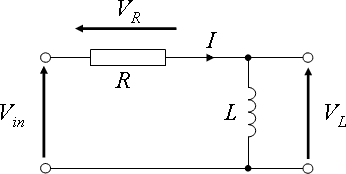
\includegraphics[width=0.5\linewidth]{Series-RL}
			%			\caption{}
			\label{fig:Series-RL}
		\end{figure}
		%
		We can model it as a first order differential equation (ODE):
		%
		\begin{equation}
			L \frac{dI}{dt} + IR = V(t)
		\end{equation}
	%
	where $L$ is inductance, $I$ is current in the circuit, $R$ is the resistance of the resistor and $V$ is the voltage of source (input / battery, etc).
	}
		
	\end{flushleft}
\end{frame}



\begin{frame}{RL: short circuit, 1}
	%\framesubtitle{How do we know the state?}
	\begin{flushleft}
		
			Short circuit equation takes form:
		
			\begin{equation}
				L \frac{dI}{dt} + IR = 0
			\end{equation}
		
			Or equivalently:
			
			\begin{equation}
				\frac{d}{dt} I =  -\frac{R}{L} I
			\end{equation}
			
			We can easily solve it:
			
			\begin{equation}
				I(t) = I_0 e^{ -\frac{R}{L} t  }
			\end{equation}
		%
		where $I_0 = I(0)$.
			
		
	\end{flushleft}
\end{frame}



\begin{frame}{RL: short circuit, 2}
	%\framesubtitle{How do we know the state?}
	\begin{flushleft}
		
		We can make some observations:
		
		\bigskip
		
		\begin{itemize}
			\item System's eigenvalue is $ -\frac{R}{L}$. It is \emph{always} negative (since $L>0$ and $R>0$), the system is asymptotically stable.
			
			\item Current $I(t)$ exponentially decays from the initial value to zero.
			
			\item The larger the inductance $L$ the slower the exponential decay. The larger the resistance $R$ the faster the decay.
			
		\end{itemize}
		
		
	\end{flushleft}
\end{frame}




\begin{frame}{RL: voltage input}
	%\framesubtitle{How do we know the state?}
	\begin{flushleft}
		
		Given a voltage input, the ODE describing an RL circuit becomes:
		
		\begin{equation}
			L \frac{dI}{dt} + IR = V(t)
		\end{equation}
	
		Analytical solution for this equation is:
		
		\begin{equation}
			I(t) = I_0 e^{ -(\frac{R}{L} t)  } + e^{ -(\frac{R}{L} t)  } \int_0^t e^{ (\frac{R}{L} \tau)  } V(\tau) d\tau
		\end{equation}
		
		
	\end{flushleft}
\end{frame}




\begin{frame}{RL: steady state, constant input}
	%\framesubtitle{How do we know the state?}
	\begin{flushleft}
		
		Given a constant input voltage $V = \text{const}$, the steady-state of the circuit ($\frac{dI}{dt} = 0$) is described as:
		
		\begin{equation}
			IR = V
		\end{equation}
		
		Giving us a steady-state solution:
		
		\begin{equation}
			I = V/R
		\end{equation}
		
		Notice that inductance $L$ does not influence the steady-state solution.
		
		
	\end{flushleft}
\end{frame}


\begin{frame}{RL: steady state, harmonic input, 1}
	%\framesubtitle{How do we know the state?}
	\begin{flushleft}
		
		Given a harmonic input voltage $V(t) = c \cos (\omega t) + d \sin (\omega t)$, we can attempt to find a steady state response of the system in the form:
		
		\begin{equation}
			I(t) = a \cos (\omega t) + b \sin (\omega t)
		\end{equation}
		
		Relations between pairs $(a, b)$ and $(c, d)$ encode the change in the phase and amplitude of the input signal.
		
		\bigskip
		
		Differentiating $I(t)$ we get:
		
		\begin{equation}
			\frac{d}{dt}I(t) = -a\omega \sin (\omega t) + b\omega \cos (\omega t)
		\end{equation}
		
	\end{flushleft}
\end{frame}




\begin{frame}{RL: steady state, harmonic input, 2}
	%\framesubtitle{How do we know the state?}
	\begin{flushleft}
		
		Substituting into the original ODE we obtain:
		
		\begin{align*}
			L\omega (-a \sin (\omega t) + b \cos (\omega t)) + \\
			+ R (a \cos (\omega t) + b \sin (\omega t))
			=
			c \cos (\omega t) + d \sin (\omega t)
		\end{align*}
	
		We can re-write it as:
		%
		\begin{align*}
			(L\omega b  + Ra  - c) \cos (\omega t)
			+
			(-L\omega a + Rb - d) \sin (\omega t) = 0
		\end{align*}
		 %
		 which would hold if:
		 
		 \begin{align}
		 	\begin{cases}
		 		 L\omega b + Ra - c = 0 \\
		 		-L\omega a + Rb - d = 0
		 	\end{cases}
		 \end{align}
		 
		
	\end{flushleft}
\end{frame}




\begin{frame}{RL: steady state, harmonic input, 3}
	%\framesubtitle{How do we know the state?}
	\begin{flushleft}
		
		We can re-write the last expression as:
		%
		\begin{align}
			\begin{cases}
				L\omega b + Ra = c  \\
				-L\omega a + Rb = d
			\end{cases}
		\end{align}
	
		Or in a matrix form:
	    %
		\begin{align}
			\begin{bmatrix}
				R & L\omega \\
				-L\omega & R
			\end{bmatrix}
			\begin{bmatrix}
				a \\ b
			\end{bmatrix}
			=
			\begin{bmatrix}
				c \\ d
			\end{bmatrix}
		\end{align}
		
		To find the expressions for $(a, b)$ we find inverse of the matrix:
		%
		\begin{align}
			\begin{bmatrix}
				R & L\omega \\
				-L\omega & R
			\end{bmatrix}^{-1}
		=
		\frac{1}{R^2 + L^2 \omega^2}
			\begin{bmatrix}
				R & -L\omega \\
				L\omega & R
			\end{bmatrix}		
		\end{align}
		
		
	\end{flushleft}
\end{frame}



\begin{frame}{RL: steady state, harmonic input, 4}
	%\framesubtitle{How do we know the state?}
	\begin{flushleft}
		
		Now we can find $(a, b)$:
		%
		\begin{align*}
			\begin{bmatrix}
				a \\ b
			\end{bmatrix}
			=
			\frac{1}{R^2 + L^2 \omega^2}
			\begin{bmatrix}
				R & -L\omega \\
				L\omega & R
			\end{bmatrix}		
			\begin{bmatrix}
				c \\ d
			\end{bmatrix}
		=
		\frac{1}{R^2 + L^2 \omega^2}
		\begin{bmatrix}
			Rc - L\omega d \\
			L\omega c + R d
		\end{bmatrix}		
		\end{align*}
	
		With that, we can find how amplitude of the output sine wave $\mathbf{amp}(I(t)) = \sqrt{a^2 + b^2}$ depends on the amplitude of the input sine wave $\mathbf{amp}(V(t)) = \sqrt{c^2 + d^2}$:
		%
		\begin{align*}
			\sqrt{a^2 + b^2}
			&=
			\frac{\sqrt{(Rc - L\omega d)^2 + (L\omega c + R d)^2}}{R^2 + L^2 \omega^2}= \\
			&= \frac{\sqrt{R^2 c^2 + L^2\omega^2 d^2 + L^2\omega^2 c^2+ R^2 d^2}}{R^2 + L^2 \omega^2}=
			\\
			&= \frac{\sqrt{(R^2+ L^2\omega^2) (c^2 + d^2) }}{R^2 + L^2 \omega^2}
			=
			\frac{1}{\sqrt{R^2 + L^2 \omega^2}} \sqrt{c^2 + d^2}
		\end{align*}
		
		
		
	\end{flushleft}
\end{frame}



\begin{frame}{RL: steady state, harmonic input, 5}
	%\framesubtitle{How do we know the state?}
	\begin{flushleft}
		
		Thus, we have the \emph{amplitude gain} $G(\omega)$:
		
		\begin{equation}
			G(\omega) = \frac{1}{\sqrt{R^2 + L^2 \omega^2}}
		\end{equation}
		
		\begin{align}
			\mathbf{amp}(I(t)) 
			=
			\frac{1}{\sqrt{R^2 + L^2 \omega^2}} \mathbf{amp}(V(t)) 
		\end{align}
	
		This is called frequency response. We can plot the amplitude gain $G(\omega)$ as a function of frequency $\omega$.
		
		
	\end{flushleft}
\end{frame}





\begin{frame}{RL: steady state, harmonic input, 6}
	%\framesubtitle{How do we know the state?}
	\begin{flushleft}
		
		Voltage $V_R$ across the resistor is given as $V_R = IR$. Therefore, the amplitude gain $G_R(\omega) = \mathbf{amp}(V_R(t)) / \mathbf{amp}(V(t)) $ of the voltage $V_R$ is:
		
		\begin{align}
			G_R(\omega)
			=
			\frac{R}{\sqrt{R^2 + L^2 \omega^2}} 
		\end{align}
	
		Voltage $V_L$ across the inducer is given as $V_L = L \frac{d}{dt}I(t)$. Its amplitude is given as $\mathbf{amp}(V_L(t)) = L\omega\sqrt{a^2 + b^2}$:
		
		\begin{align}
			G_R(\omega)
			=
			\frac{L\omega}{\sqrt{R^2 + L^2 \omega^2}} 
		\end{align}
		
	\end{flushleft}
\end{frame}



\begin{frame}{RL: steady state, harmonic input, 7}
	%\framesubtitle{How do we know the state?}
	\begin{flushleft}
		
		Analyzing the amplitude gain $G(\omega) = \frac{1}{\sqrt{R^2 + L^2 \omega^2}}$ we can see that:
		
		\bigskip
		
		\begin{itemize}
			\item As frequency tends to infinity, the gain goes to zero.
			
			\item As frequency tends to zero, the gain goes to $1/R$.
		\end{itemize}
	
		\bigskip
		
		This makes RL circuit a \emph{low-pass filter}: high-frequency signals are attenuated (suppressed) by the circuit.
		
	\end{flushleft}
\end{frame}


\begin{frame}{Laplace transform}
	%\framesubtitle{How do we know the state?}
	\begin{flushleft}
		
		By definition, Laplace transform of a function $f(t)$ is given as:
		
		\begin{equation}
			F(s) = \int_0^\infty f(t) e^{-st}dt
		\end{equation}
		
		\bigskip
		
		In particular, Laplace transform of a derivative $\frac{d}{dt}x(t)$ is $s X(s)$.
		
	\end{flushleft}
\end{frame}




\begin{frame}{RL: Laplace transform}
	%\framesubtitle{How do we know the state?}
	\begin{flushleft}
		
		Time domain ODE for the RL circuit is:
		
		\begin{equation}
			L \frac{dI}{dt} + IR = V(t)
		\end{equation}
		
		Laplace transform of this equation is:
		
		\begin{equation}
			Ls I(s) + I(s)R = V(s)
		\end{equation}
		%
		where $I(s)$ and $V(s)$ are Laplace transform of current $I(t)$ and voltage $V(t)$.
	
	\end{flushleft}
\end{frame}



\begin{frame}{RL: Transfer functions}
	%\framesubtitle{How do we know the state?}
	\begin{flushleft}
		
		Laplace domain ODE is $Ls I(s) + I(s)R = V(s)$. The transfer function from $V(s)$ to $I(s)$ is $I(s) = W_I(s)V(s)$:
		
		\begin{equation}
			W_I(s) = \frac{1}{Ls + R}
		\end{equation}
		
		Voltage across the resistor $V_R = IR$ can be computed via its transfer function $V_R(s) = W_R(s) V(s)$:
		
		\begin{equation}
			W_R(s) = \frac{R}{Ls + R}
		\end{equation}
	
		Voltage across the inducer $V_L(s) = Ls I(s)$ can be computed via its transfer function $V_L(s) = W_L(s) V(s)$:
	
		\begin{equation}
			W_L(s) = \frac{Ls}{Ls + R}
		\end{equation}

	\end{flushleft}
\end{frame}



\begin{frame}{RL: Frequency response, 1}
	%\framesubtitle{How do we know the state?}
	\begin{flushleft}
		
		Knowing transfer function $W(s)$, we can compute frequency response by substituting $\omega j$ for $s$ into the transfer function and finding its absolute value. Doing it for the transfer function $W_I(s) = \frac{1}{Ls + R}$ we get:
		
		\begin{align}
			W_I(\omega) = \frac{1}{L\omega j + R} =
			 \frac{-L\omega j + R}{L^2\omega^2 + R^2}; \\
			|W_I(\omega)| = \frac{\sqrt{L^2\omega^2 + R^2}}{L^2\omega^2 + R^2} =
			\frac{1}{\sqrt{L^2\omega^2 + R^2}}
		\end{align}
		
	\end{flushleft}
\end{frame}


\begin{frame}{RL: Frequency response, 2}
	%\framesubtitle{How do we know the state?}
	\begin{flushleft}
		
		Same for the transfer function $W_R(s) = \frac{R}{Ls + R} = R W_I(s) $ yields:
		
		\begin{align}
			|W_R(\omega)| = 
			\frac{R}{\sqrt{L^2\omega^2 + R^2}}
		\end{align}
	
		Considering transfer function $W_L(s) = \frac{Ls}{Ls + R}$ yields:
		
		\begin{align*}
			W_L(\omega) = \frac{L\omega j}{L\omega j + R} =
			\frac{L^2\omega^2 + RL\omega j}{L^2\omega^2 + R^2}; \\
			|W_L(\omega)| = \frac{\sqrt{L^4\omega^4 + R^2L^2\omega^2}}{L^2\omega^2 + R^2} =
			L\omega\frac{\sqrt{L^2\omega^2 + R^2}}{L^2\omega^2 + R^2} =
			\frac{L\omega}{\sqrt{L^2\omega^2 + R^2}}
		\end{align*}
	
		Thus, we found frequency responses from earlier without solving the ODEs.
		
	\end{flushleft}
\end{frame}





\begin{frame}{RC circuit}
	%\framesubtitle{How do we know the state?}
	\begin{flushleft}
		
		Consider RC circuit (resistor-capacitor circuit):
		%
\begin{figure}
	\centering
	\begin{subfigure}[b]{0.5\textwidth}
		\centering
		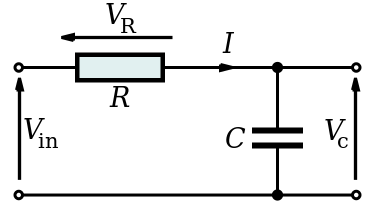
\includegraphics[width=\textwidth]{RC_1}
		\caption{Voltage input}
%		\label{fig:y equals x}
	\end{subfigure}
	\begin{subfigure}[b]{0.3\textwidth}
		\centering
		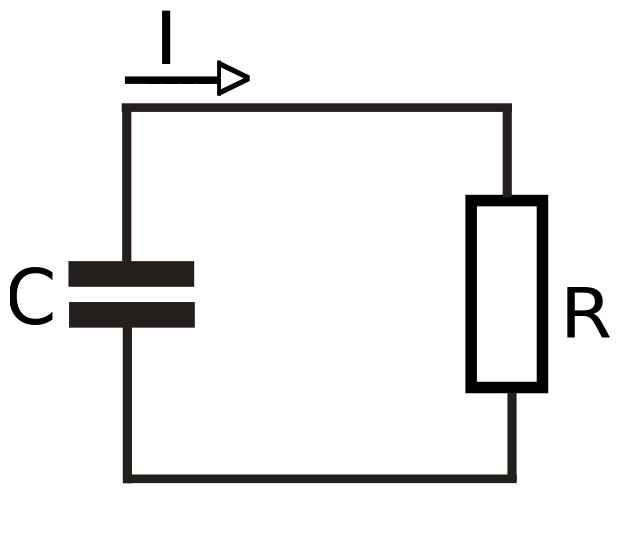
\includegraphics[width=\textwidth]{RC_2}
		\caption{Short circuit}
%		\label{fig:three sin x}
	\end{subfigure}
%	\caption{Three simple graphs}
%	\label{fig:three graphs}
\end{figure}
		
	\end{flushleft}
\end{frame}



\begin{frame}{RC circuit ODE}
	%\framesubtitle{How do we know the state?}
	\begin{flushleft}
		
		We can define electric charge of a capacitor as $q$, relating to the current as:
		
		\begin{equation}
			q(t) = q(0) + \int_0^{t} I(\tau) d\tau
		\end{equation}
		
		This means that $\frac{dq(t)}{dt} = I(t)$.
		
		\bigskip
		
		Voltage across the capacitor is $V(t) = \frac{q(t)}{C}$. This gives us ODE of the circuit:
		
		\begin{equation}
			\frac{q(t)}{C} + I(t)R = V(t)
		\end{equation}
		
		Which is the same as:
		
		\begin{equation}
			\frac{q(t)}{C} + \frac{dq(t)}{dt} R = V(t)
		\end{equation}
		
		
	\end{flushleft}
\end{frame}



\begin{frame}{RC circuit Laplace Transform}
	%\framesubtitle{How do we know the state?}
	\begin{flushleft}
		
		Expression $\frac{dq(t)}{dt} = I(t)$ in Laplace domain becomes $s q(s) = I(s)$. Dividing by $s$ we get:
		
		\begin{equation}
			q(s) = \frac{1}{s} I(s)
		\end{equation}
		
		Note that $1/s$ is a representation of an \emph{integrator} in Laplace domain. So, the time domain equation $\frac{q(t)}{C} + I(t)R = V(t)$ becomes:
		
		\begin{equation}
			\frac{1}{sC}I(s) + I(s)R = V(s)
		\end{equation}
		
		Giving us a transfer function:
		
		\begin{equation}
			I(s) =  \frac{sC}{1 + sCR}V(s)
		\end{equation}
		
		
	\end{flushleft}
\end{frame}


\begin{frame}{RC circuit, Transfer functions}
	%\framesubtitle{How do we know the state?}
	\begin{flushleft}
		
		The transfer function from input voltage $V(s)$ to current $I(s)$ is $I(s) =  W_I(s)V(s)$
		
		\begin{equation}
			W_I(s) = \frac{sC}{1 + sCR}
		\end{equation}
		
		The transfer function from input voltage $V(s)$ to voltage across the resistor $V_R(s) = I(s) R$ is:
		
		\begin{equation}
			W_R(s) = \frac{sCR}{1 + sCR}
		\end{equation}
	
		The transfer function from input voltage $V(s)$ to voltage across the capacitor $V_C(s) = \frac{1}{sC}I(s)$ is:
	
		\begin{equation}
		W_C(s) = \frac{1}{1 + sCR}
		\end{equation}
		
		
	\end{flushleft}
\end{frame}



\begin{frame}{RC circuit, frequency response}
	%\framesubtitle{How do we know the state?}
	\begin{flushleft}
		
		The frequency response of the voltage across the capacitor is found by substituting $\omega j$ into $W_C(s)$
		
		\begin{align}
			W_C(\omega) = \frac{1}{1 + CR\omega j} = \frac{1 - CR\omega j}{1 + C^2 R^2 \omega^2} \\
			| W_C(\omega) | = \frac{\sqrt{1 + C^2 R^2 \omega^2}}{1 + C^2 R^2 \omega^2} 
			= \frac{1}{\sqrt{1 + C^2 R^2 \omega^2}} 
		\end{align}
		
		The frequency response of the voltage across the resistor is found by substituting $\omega j$ into $W_R(s)$
		
		\begin{align*}
			W_R(\omega) = \frac{CR\omega j}{1 + CR\omega j} = \frac{CR\omega j + C^2R^2\omega^2}{1 + C^2 R^2 \omega^2} = CR\omega\frac{ j + CR\omega}{1 + C^2 R^2 \omega^2} \\
			| W_R(\omega) | 
			=  \frac{ CR\omega}{\sqrt{1 + C^2 R^2 \omega^2}} 
		\end{align*}
		
	\end{flushleft}
\end{frame}



\begin{frame}{RC: filter}
	%\framesubtitle{How do we know the state?}
	\begin{flushleft}
		
		Analyzing the amplitude gain $| W_R(\omega) | 
		=  \frac{ CR\omega}{\sqrt{1 + C^2 R^2 \omega^2}} $ we can see that:
		
		\bigskip
		
		\begin{itemize}
			\item As frequency tends to infinity, the gain goes to 1.
			
			\item As frequency tends to zero, the gain goes to 0.
		\end{itemize}
		
		\bigskip
		
		This makes RL circuit a \emph{high-pass filter}: low-frequency signals are attenuated (suppressed) by the circuit.
		
	\end{flushleft}
\end{frame}



\begin{frame}{RLC circuit ODE, 1}
	%\framesubtitle{How do we know the state?}
	\begin{flushleft}
		
		Remember that voltage across the capacitor is $V_C(t) = \frac{q(t)}{C}$, and voltage across an inducer is $V_L(t) = L \frac{d}{dt}I(t)$. This gives us ODE of the circuit:
		
		\begin{equation}
			L \frac{d}{dt}I(t) + \frac{q(t)}{C} + I(t)R = V(t)
		\end{equation}
	
		In Laplace domain these equalities are $V_C(s) = \frac{1}{sC} I(s)$ and $V_L(s) = sLI(s)$:
		
		\begin{align}
			 sLI(s) + RI(s) + \frac{1}{sC} I(s) = V(s) \\
			 \frac{s^2LC}{sC}I(s) + \frac{sCR}{sC}I(s) + \frac{1}{sC} I(s) = V(s) \\
			 I(s) = \frac{sC}{s^2 LC + s RC + 1} V(s)
		\end{align}
		
		
	\end{flushleft}
\end{frame}



\begin{frame}{RLC circuit ODE, 2}
	%\framesubtitle{How do we know the state?}
	\begin{flushleft}
		
		Alternative ways to describe RLC circuit dynamics is:
		
		\begin{equation}
			L \frac{d}{dt}I(t) + I(t)R + \frac{1}{C} \int_0^{t} I(\tau) d\tau = V(t)
		\end{equation}
		
		\begin{equation}
			\left(s^2 + \frac{R}{L}s + \frac{1}{LC} \right)I(s) = sV(s)
		\end{equation}
		
		The voltage across the conductor is $V_C(s) = \frac{1}{sC} I(s)$:
		%
		\begin{align}
			V_C(s) = \frac{1}{s^2 LC + s RC + 1} V(s)
		\end{align}
		
		The voltage across the inducer is $V_L(s) = sLI(s)$:
		%
		\begin{align}
			V_L(s) = \frac{s^2 LC}{s^2 LC + s RC + 1} V(s)
		\end{align}
				
	\end{flushleft}
\end{frame}



\myqrframe

\end{document}
